	

% microtype: Tipografía.
% mathpazo: Usa la fuente Palatino.
\documentclass[a4paper, 11pt]{article}
\usepackage[protrusion=true,expansion=true]{microtype}
\usepackage{mathpazo}
\usepackage{booktabs}
\usepackage{multicol}
\usepackage{multirow}
\usepackage{algorithm}
\usepackage{algpseudocode}	
\usepackage{amsmath}





\makeatletter
\def\BState{\State\hskip-\ALG@thistlm}
\makeatother


% Indentación de párrafos para Palatino
\setlength{\parindent}{0pt}
  \parskip=8pt
\linespread{1.05} % Change line spacing here, Palatino benefits from a slight increase by default


%%% Castellano.
% noquoting: Permite uso de comillas no españolas.
% lcroman: Permite la enumeración con numerales romanos en minúscula.
% fontenc: Usa la fuente completa para que pueda copiarse correctamente del pdf.
\usepackage[spanish,es-noquoting,es-lcroman]{babel}
\usepackage[utf8]{inputenc}
\usepackage[T1]{fontenc}
\selectlanguage{spanish}


%%% Gráficos
\usepackage{graphicx} % Required for including pictures
\usepackage{wrapfig} % Allows in-line images
\usepackage[usenames,dvipsnames]{color} % Coloring code


%%% Matemáticas
\usepackage{amsmath}
\usepackage[hidelinks]{hyperref}
%%% Código


\usepackage{listings}

%% Listing settings

\usepackage{color}

\definecolor{dkgreen}{rgb}{0,0.6,0}
\definecolor{gray}{rgb}{0.5,0.5,0.5}
\definecolor{mauve}{rgb}{0.58,0,0.82}

\lstset{frame=tb,
  language=Java,
  aboveskip=3mm,
  belowskip=3mm,
  showstringspaces=false,
  columns=flexible,
  basicstyle={\small\ttfamily},
  numbers=none,
  numberstyle=\tiny\color{gray},
  keywordstyle=\color{blue},
  commentstyle=\color{dkgreen},
  stringstyle=\color{mauve},
  breaklines=true,
  breakatwhitespace=true,
  tabsize=3
}



%%% Bibliografía
\makeatletter
\renewcommand\@biblabel[1]{\textbf{#1.}} % Change the square brackets for each bibliography item from '[1]' to '1.'
\renewcommand{\@listI}{\itemsep=0pt} % Reduce the space between items in the itemize and enumerate environments and the bibliography



%----------------------------------------------------------------------------------------
%	TÍTULO
%----------------------------------------------------------------------------------------
% Configuraciones para el título.
% El título no debe editarse aquí.
\renewcommand{\maketitle}{
  \begin{flushright} % Right align
  
  {\LARGE\@title} % Increase the font size of the title
  
  \vspace{50pt} % Some vertical space between the title and author name
  
  {\large\@author} % Author name
  \\\@date % Date
  \vspace{40pt} % Some vertical space between the author block and abstract
  \end{flushright}
}

%% Título
\title{\textbf{Memoria de la práctica 4}\\ % Title
Algorítmica} % Subtitle

\author{\textsc{Fco. Javier Sáez Maldonado}\\ % Author
\textsc{Laura Gómez Garrido}\\
\textsc{Luis Antonio Ortega Andrés}\\
\textsc{Pedro Bonilla Nadal}\\
\textsc{Daniel Pozo Escalona}\vspace{2cm}
\\{\textit{Universidad de Granada}}} % Institution

\date{\today} % Date



%----------------------------------------------------------------------------------------
%	DOCUMENTO
%----------------------------------------------------------------------------------------

\begin{document}

\maketitle % Print the title section


%% Índice
{\parskip=2pt
  \tableofcontents
}
\pagebreak

%%% Inicio del documento


\section{Problema}
 Referencia: El puzzle “\textbf{La Maleta de Luke}” (El Profesor Layton y la Caja de
Pandora, Nintendo DS).


Diversos videojuegos de la categoría puzzle ofrecen rompecabezas que pueden
ser estudiados como un problema de exploración en grafos. En particular, el puzzle “La maleta de Luke” presentado en El profesor Layton y la Caja de Pandora para Nintendo DS, supone que hay una maleta y diversos objetos que tenemos que introducir en ella
sin que se solapen, cada uno de unas dimensiones determinadas.
Estos problemas se pueden discretizar, de modo que en nuestro caso dividiremos
la maleta en un rectángulo de 6 casillas de alto por 9 de ancho, y cada objeto también lo
discretizaremos con estas mismas dimensiones:\\
\begin{center}
	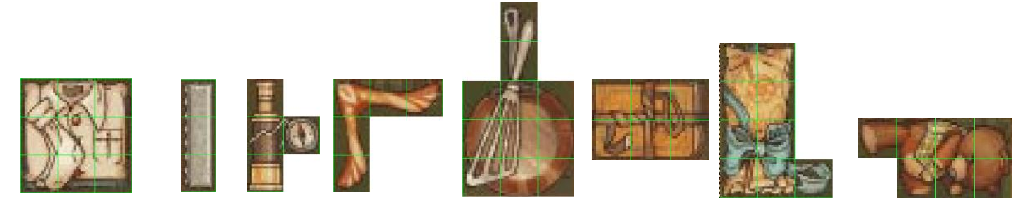
\includegraphics[scale=0.35]{piezas.png}
\end{center}

Cada pieza, a la hora de colocarla en una posición de la maleta, puede
rotarse 0º, 90º, 180º o 270º para alcanzar la solución. De este modo, el
puzzle se resuelve colocando las piezas según la siguiente figura:
\begin{center}
	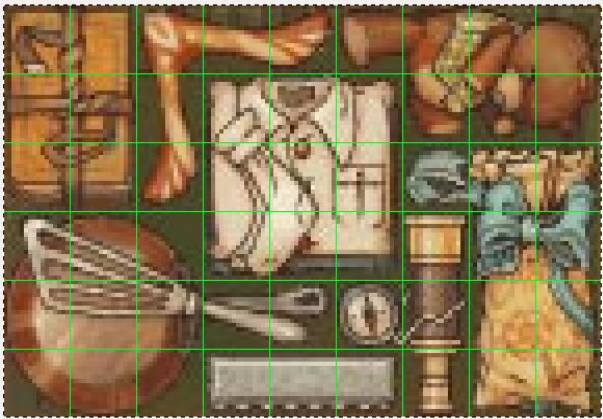
\includegraphics[scale=0.35]{solucion.png}
\end{center}


Se pide diseñar e implementar un algoritmo de exploración en grafos
(BackTracking o Branch\&Bound) que solucione este problema con el tamaño de maleta
y piezas descritas en este apartado.

\section{Solución}




\subsection{Elección de la técnica}
Nuestro problema ha sido resuelto mediante la utilización de la técnica de resolución de algoritmos: "Backtracking", ya que hemos intentado buscar todas las soluciones posibles que existen y devolver la primera que nos aparezca, sin establecer qué solución es más optima ni explorar todo el espacio de las soluciones como hace "Branch and bound", que era la otra alternativa que teníamos para resolver nuestro problema.

\subsection{Diseño de la solución}
Para nuestra solución,tenemos varios elementos
\begin{itemize}
	\item Representación: $T(x_1,\cdots,x_8)$ es un vector donde cada 
componente representa una columna del tablero y cada valor de x es la fila en la que se colocará la esquina superior izquierda de una pieza.
	\item Restricciones implícitas: $x_i$ tendrá valores entre $0$ y $5$, ya que la matriz es de $6$ filas.
	\item Restricciones explícitas: Todas las piezas deben caber dentro de la  matriz sin solaparse y la matriz debe estar llena.
	\item Representación del árbol implícito: En cada nivel $i$ del árbol estará la pieza
	\item Función objetivo: Encontrar una tupla $T(x_1,\cdots, x_8)$ tal que cada posición represente una pieza y elemento de la tupla esté la posición de la esquina superior izquierda de la pieza donde esta está colocada.
	\item Función de poda: Al hacer $T(x_1,\cdots,x_{k-1}) \cup x_k$ debe cumplir que la pieza $x_k$ encaje en la posición asignada.
\end{itemize}

\section{El algoritmo}

\subsection{Esqueleto del algoritmo}

Nuestro algoritmo se puede representar mediante pseudocódigo de la siguiente manera:

\begin{algorithm}
\begin{algorithmic}
\Function{EncajarPiezasEnMaleta}{Pieza, tablero, indice}
	\If{Tablero Lleno}
		\State \Return $true$
	\EndIf
	
	\For{$i=1,\dots,4$} \Comment Rotaciones
        \For{$j = 0,\dots,FILAS$} \Comment Filas
        	\For{$k= 0, \dots,COLUMNAS$} \Comment Columnas
        	
        	\If{No cabe Pieza[indice][Rotacion i] en posición  (j,k)}
        		\State Pasamos a siguiente rotación o pieza
        	\EndIf
        	
        	\State $copiaSeguridad \gets  tablero$
        	\State Colocamos pieza donde hemos visto que cabe
        	\State $indice++$
        	\State $resuelto \gets resolver(pieza,tablero,indice)$ \Comment Llamada recursiva
        	
        	\If{Resuelto}
        		\State \Return $true$
        	
        	\Else
        		\State $tablero \gets copiaSeguridad$
        		\State $indice --$
        	
        	\EndIf
        	
        	
        	
        	\EndFor   \Comment Columnas	
      	\EndFor \Comment Filas
    \EndFor \Comment Rotaciones
	
\State \Return False \Comment Falso si no se encuentra la solución

\EndFunction
\end{algorithmic}
\end{algorithm}

Se puede ver como la técnica de BackTracking se aplica en la generación mediante la llamada recursiva de un árbol de soluciones que se va explorando hasta encontrar la solución.

\subsection{Ejemplo sencillo}

Realizaremos un ejemplo muy sencillo sobre cómo funcionaría nuestro algoritmo. Pondremos las dos primeras piezas que se mostraron al principio y una matriz(un tablero) que será el siguiente:
\[
\begin{pmatrix}
 0 & 0 & 0 \\
0 & 0 & 0\\
0 & 0 & 0\\
0 & 0 & 0 \\ 
\end{pmatrix} 
\]
Donde los ceros significarán que la posición está vacía.

Si las piezas son:
\begin{center}
	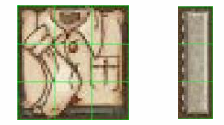
\includegraphics{ejemplo.png}
\end{center}
se puede ver que son de $3\times 3$ y $3\times 1$. Para identificarlas matricialmente, la primera será, en todas sus rotaciones:
\[
\begin{pmatrix}
1 & 1 & 1\\
1& 1 & 1\\
1 & 1 & 1
\end{pmatrix} 
\]

Y la segunda, será:
\[
\begin{pmatrix}
2\\
2\\
2
\end{pmatrix} 
\]
en su primera rotación y
\[
\begin{pmatrix}
2&2&2
\end{pmatrix} 
\]
en su segunda rotación.

Ahora, nuestro algoritmo empezaría y vería que la matriz inicial no está llena y por tanto comprobará si en la primera posición libre que haya, cabe la primera pieza. Como el resultado es afirmativo,la introducirá y quedará la matriz:
\[
\begin{pmatrix}
 1 & 1 & 1 \\
1 & 1 & 1\\
1 & 1 & 1\\
0 & 0 & 0 \\ 
\end{pmatrix} 
\]

Seguidamente, intentará seguir colocando las demás piezas para ver si se puede resolver. Pasará a la segunda pieza, habiendo hecho una copia de la matriz antes de seguir por si tiene que volver. Para seguir colocando, llamará recursivamente con la siguiente pieza.

Sigue nuestro algorimo intentando ahora introducir la pieza 2 en su primera rotación mediante la llamada recursiva. El resultado de la función cabe será falso, por lo que seguirá con la siguiente rotación. En este caso, sí podrá introducirla y la introducirá, quedando la matriz(tablero) de la forma:

\[
\begin{pmatrix}
 1 & 1 & 1 \\
1 & 1 & 1\\
1 & 1 & 1\\
2 & 2 & 2
\end{pmatrix} 
\]
que, como vemos, ya está resuelto. Aún así, volverá a llamar recursivamente sumando el índice, pero en la llamada la función llena devolverá verdadero, y así todas las llamadas recursivas devolverán verdadero y terminará la función y quedará resuelto el problema.


\section{Un caso real}

Un ejemplo en el que podríamos aplicar nuestro algoritmo sería en la construcción de un polideportivo. Al igual que en nuestro algoritmo, sabemos de antemano el espacio que tenemos, lo que queremos colocar dentro y cuánto ocupa cada uno. De esta forma, escribiendo en forma matricial el terreno y las pistas de los diferentes deportes que se quieran colocar, podríamos comprobar si estas caben o no en el espacio que tenemos y de qué forma cabrían.

\section{Cálculo del orden de eficiencia teórica}



\section{Instrucciones de compilación}

Para compilar nuestro código, en la carpeta donde se tengan los archivos, abrir la terminal y ejecutar $make$ para que se genere el ejecutable.
\end{document}
